\providecommand{\main}{../../../..}
\documentclass[\main/dresen_thesis.tex]{subfiles}
\begin{document}
  \label{sec:looselyPackedNS:layers:pnr}
  \begin{figure}[tb]
    \centering
    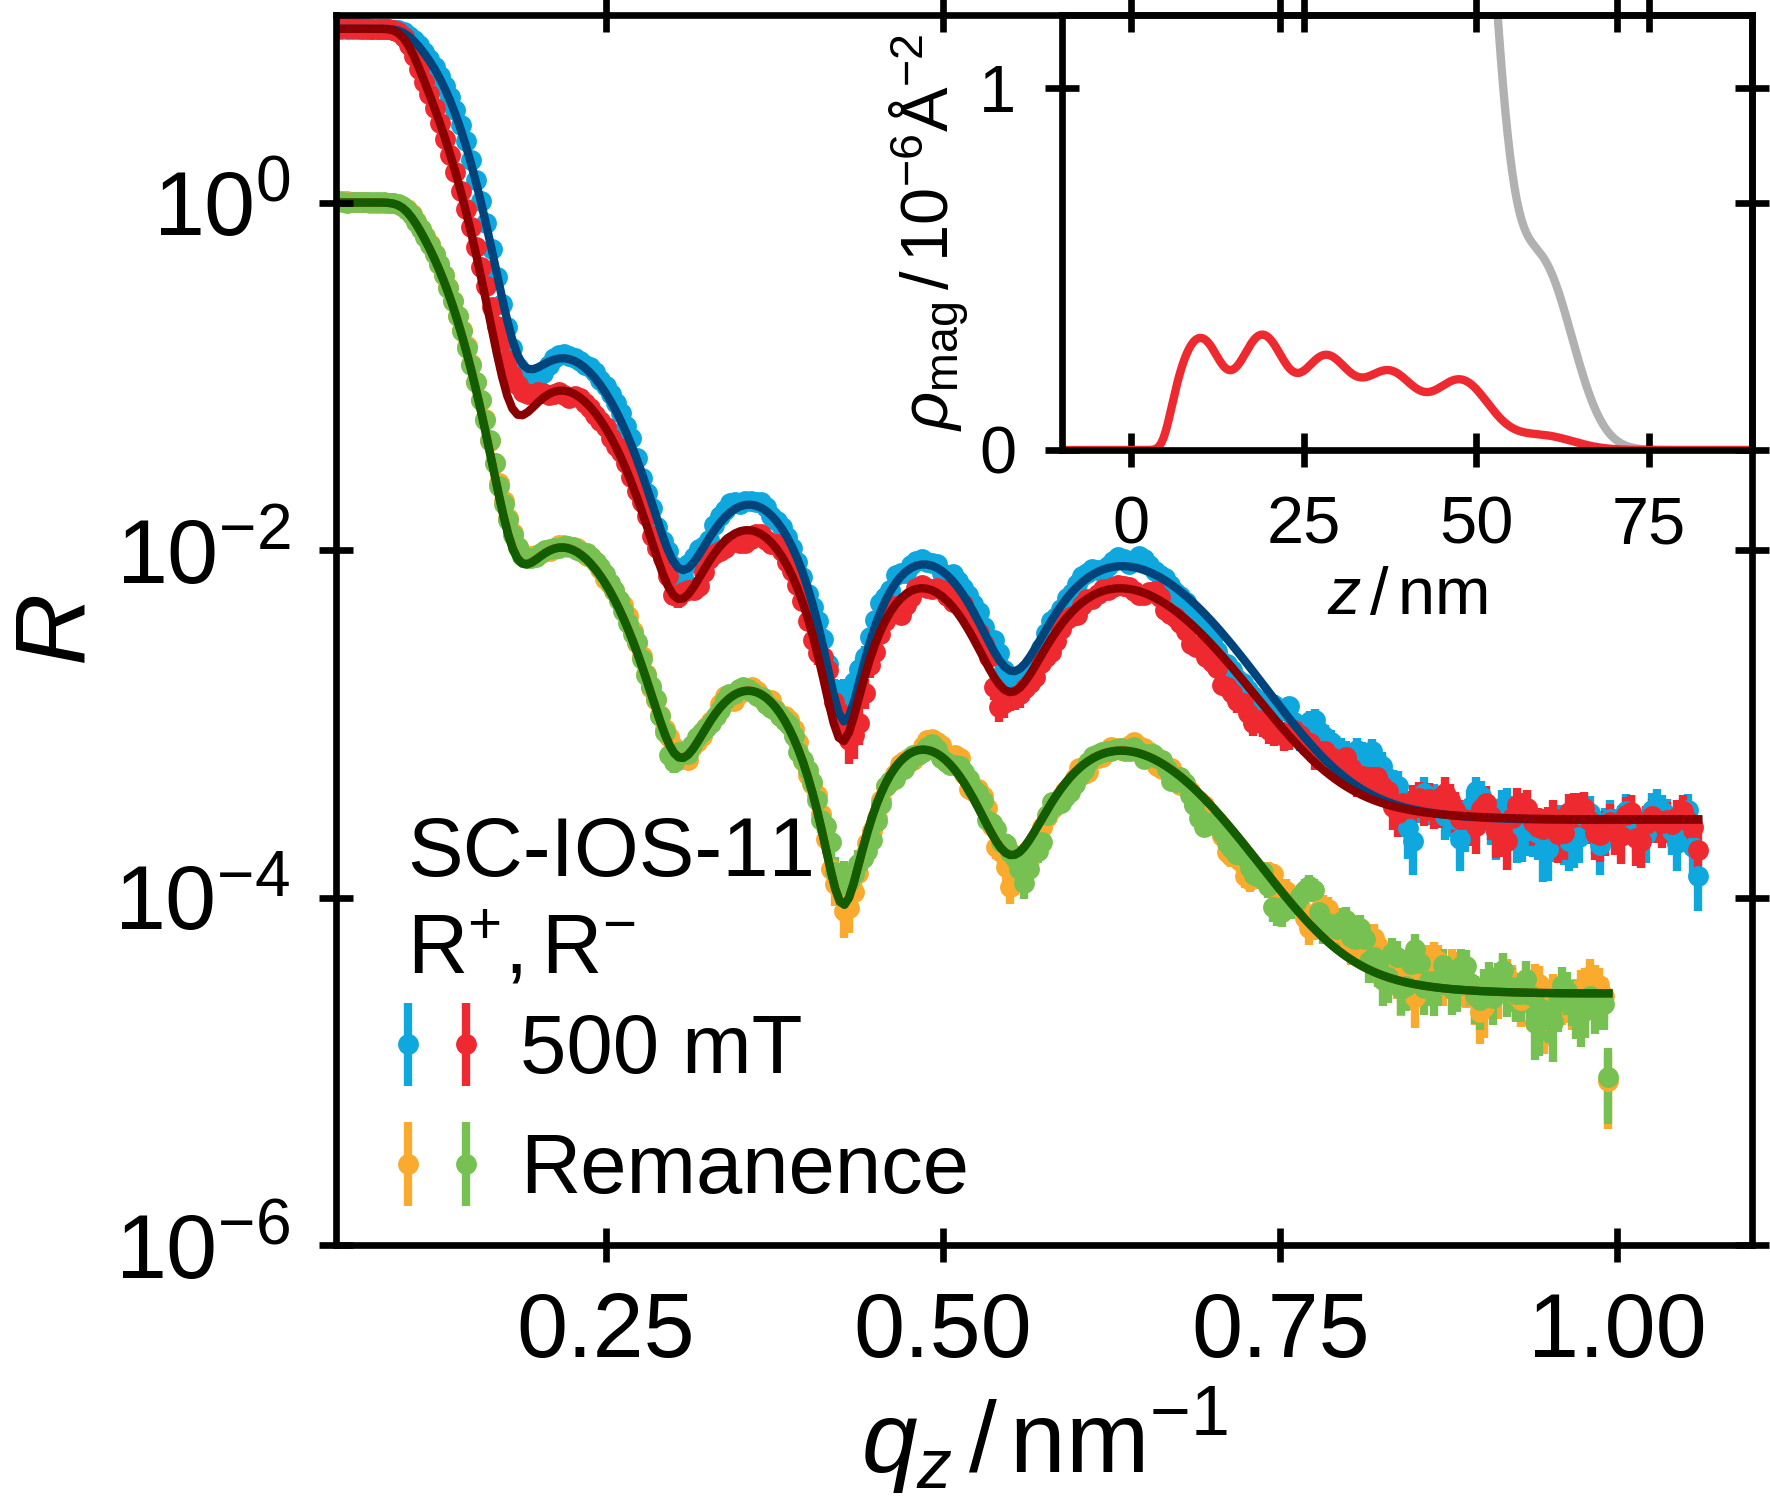
\includegraphics{looselyPackedNP_VerticalStructure_SC-IOS-11_PNR300K_500mT}
    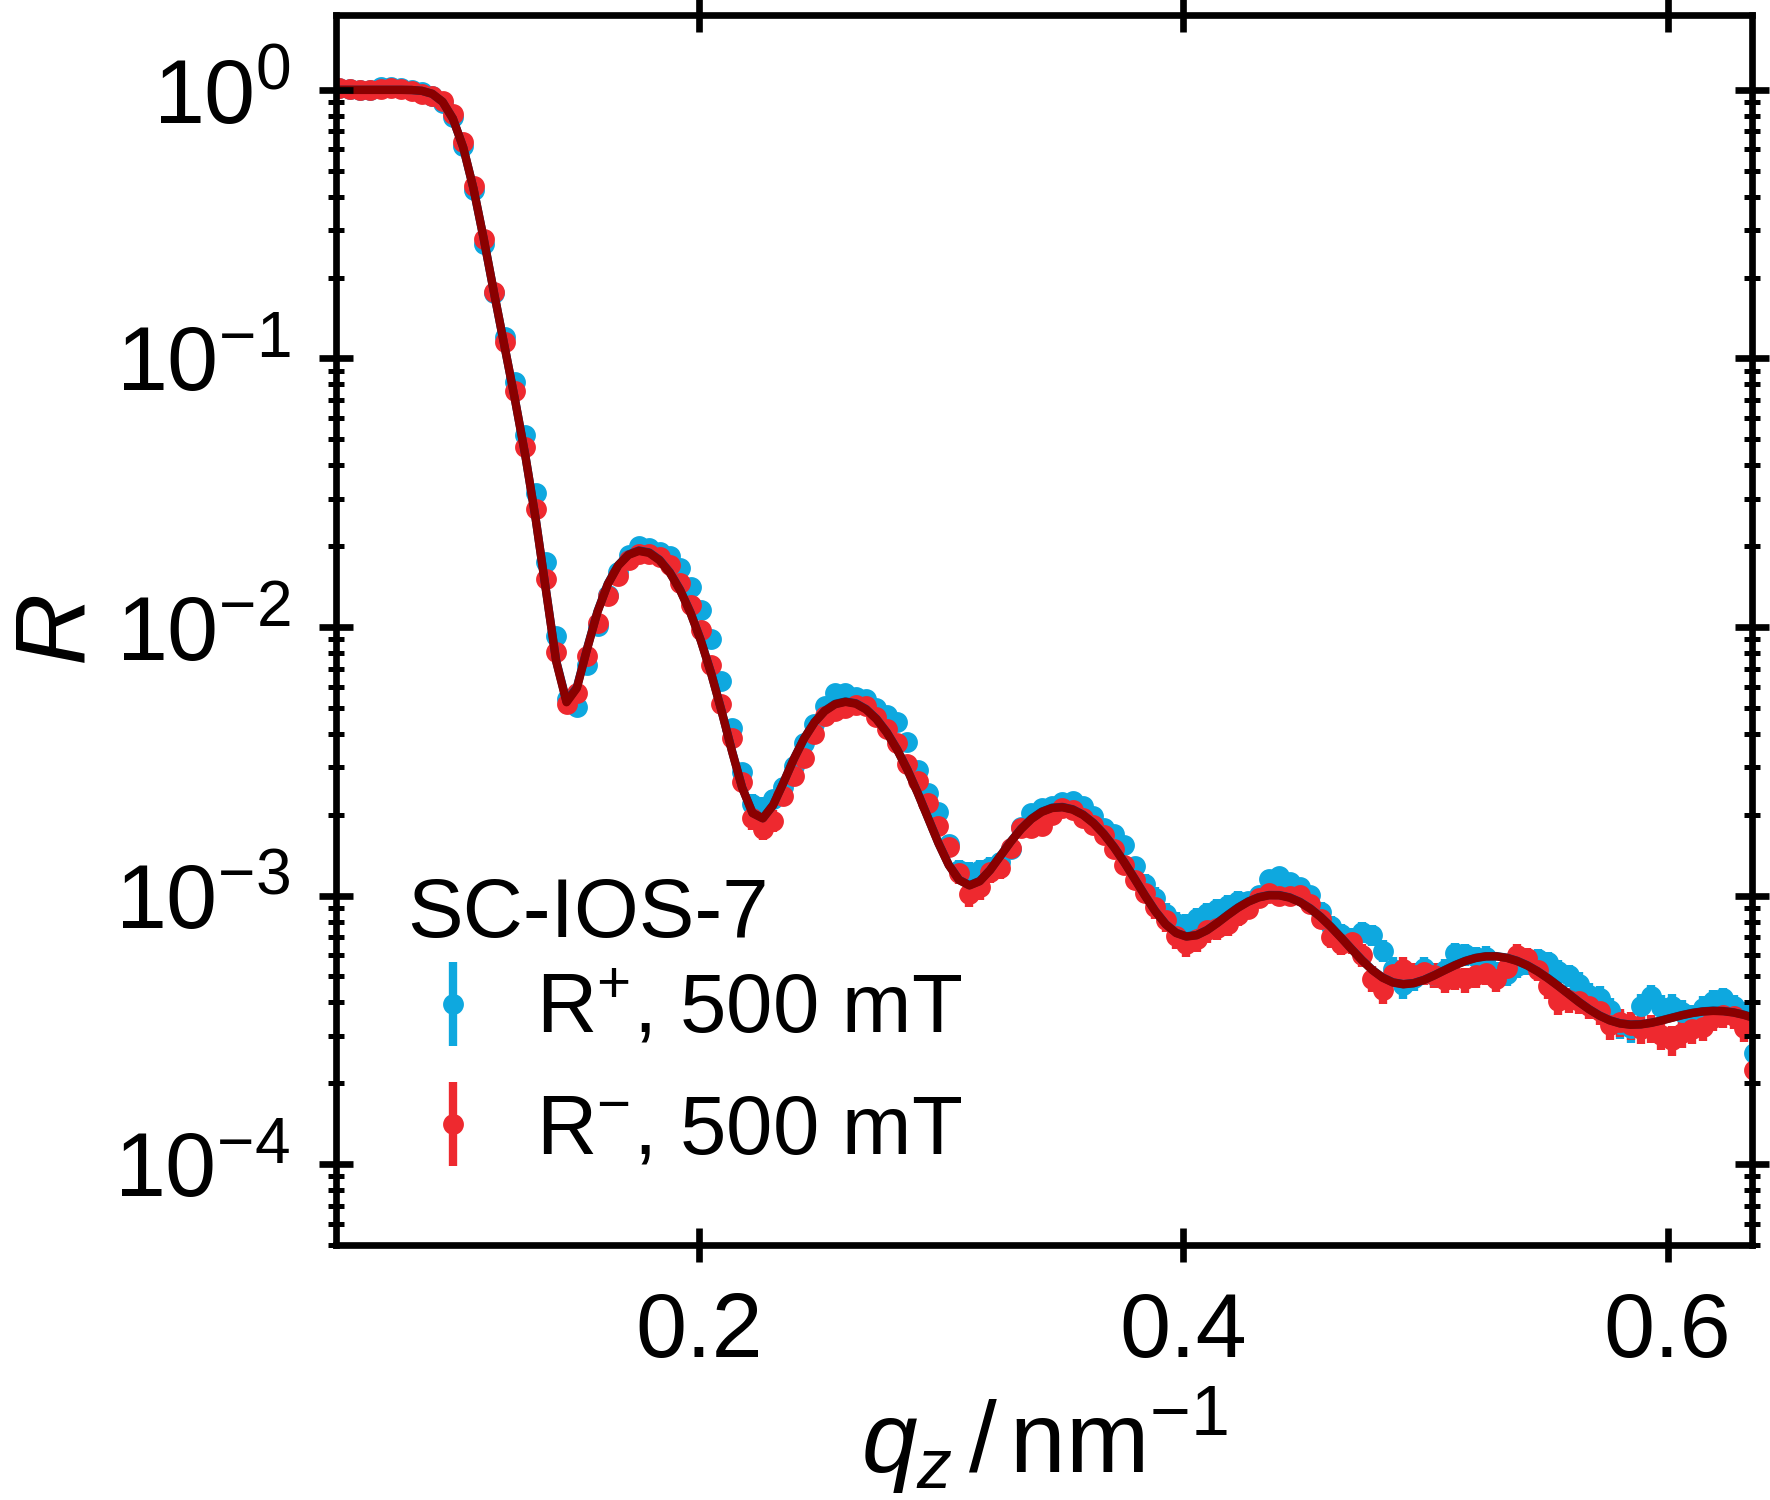
\includegraphics{looselyPackedNP_VerticalStructure_SC-IOS-7_PNR300K_500mT}
    \caption{\label{fig:looselyPackedNP:layer:pnrRoomTemperatureMagnetic}Room temperature polarized neutron reflectivity ($R^{+},\, R^{-}$) of SC-IOS-11 (left) and SC-IOS-7 (right). For SC-IOS-11 the PNR measured after removal of the field at remanence is additionally shown.}
  \end{figure}
  

  \begin{figure}[tb]
    \centering
    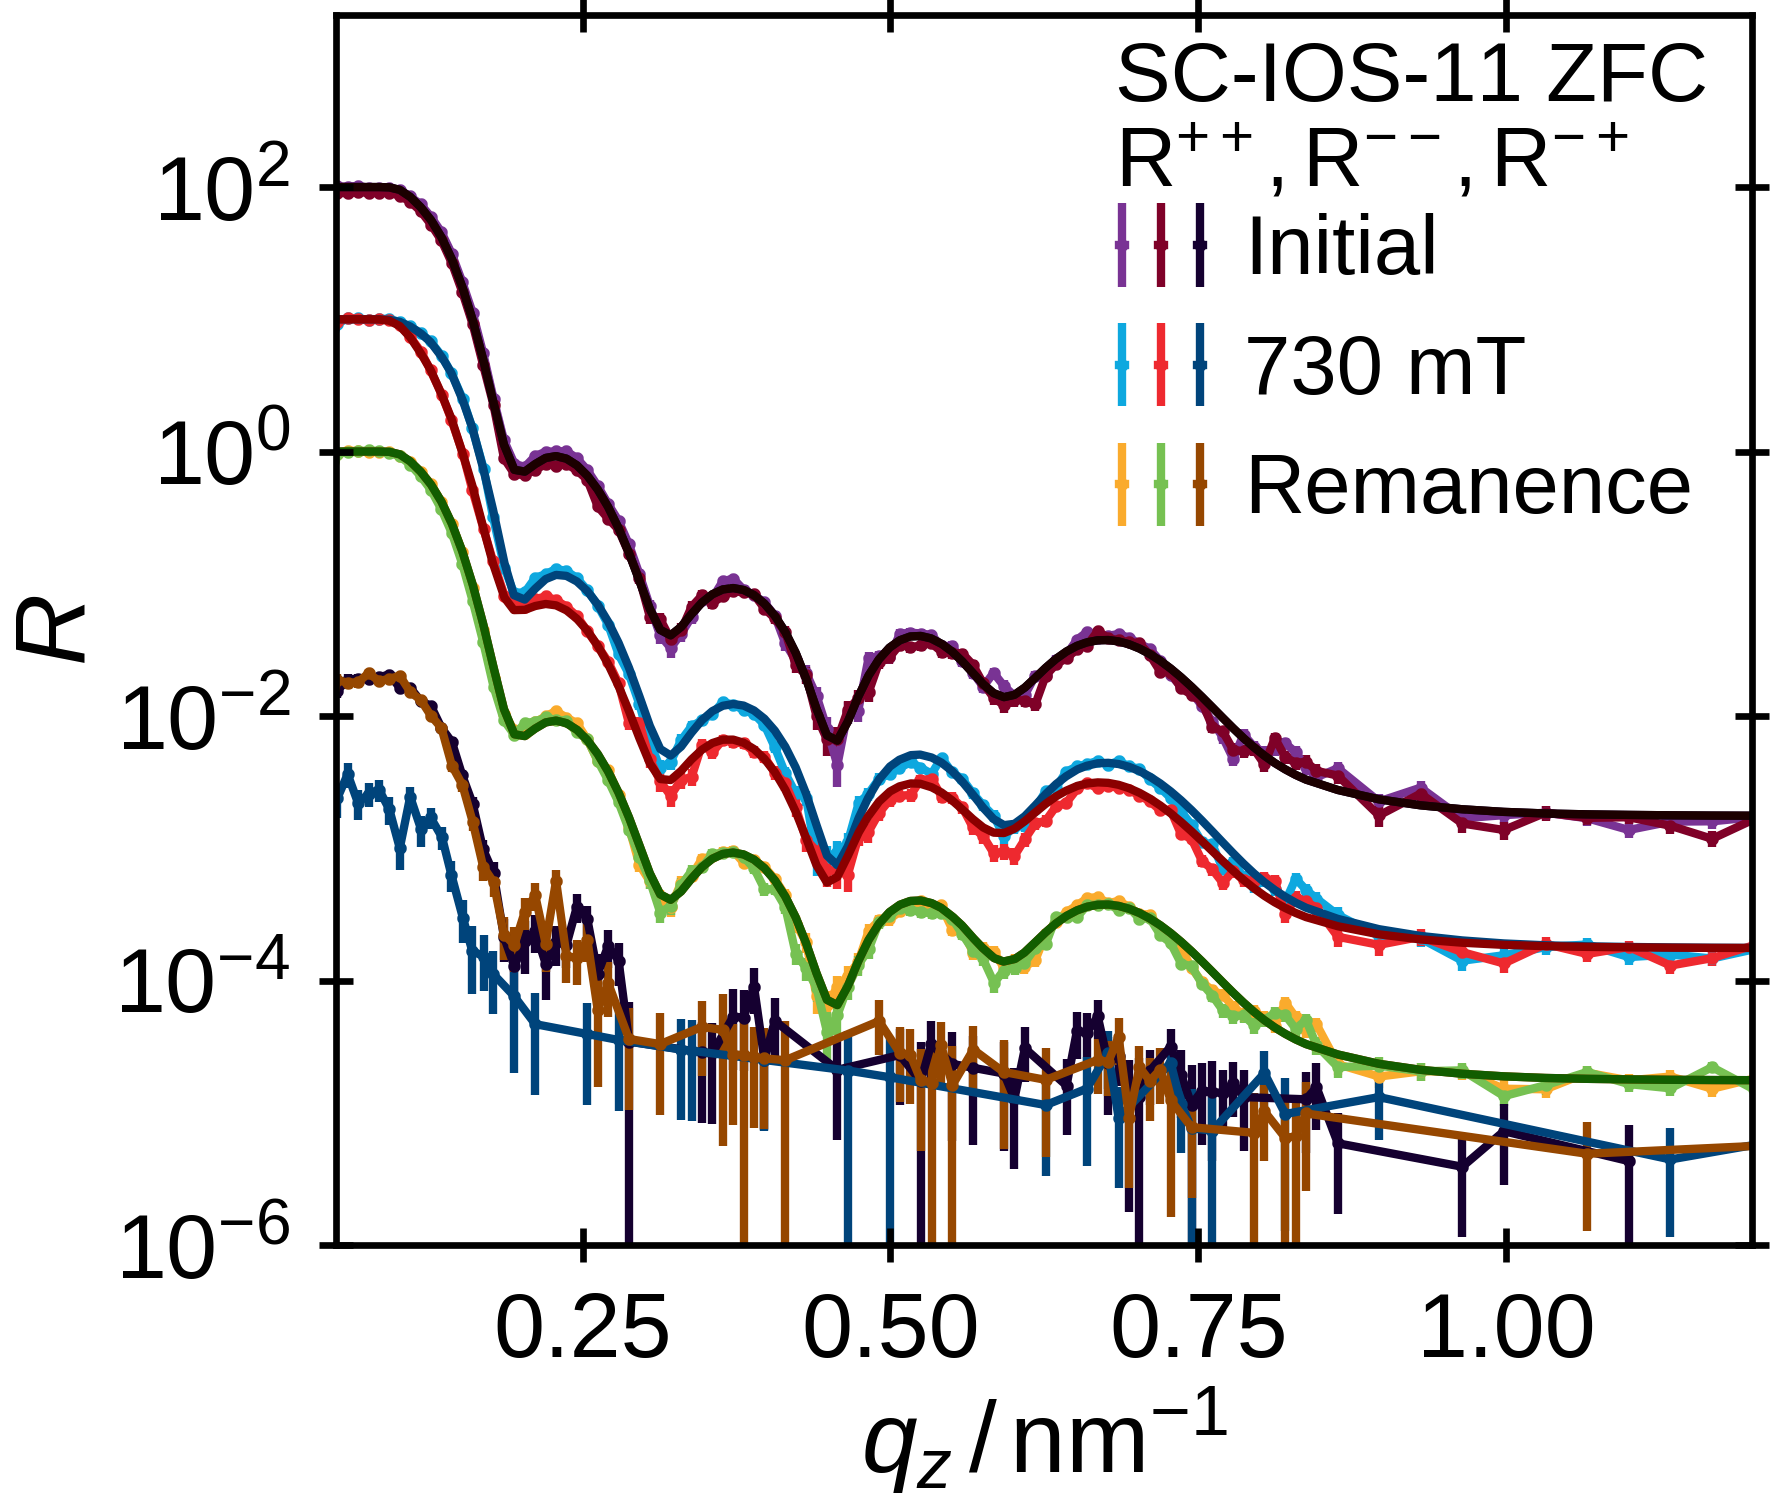
\includegraphics{looselyPackedNP_VerticalStructure_SC-IOS-11_PNR_ZFC30K}
    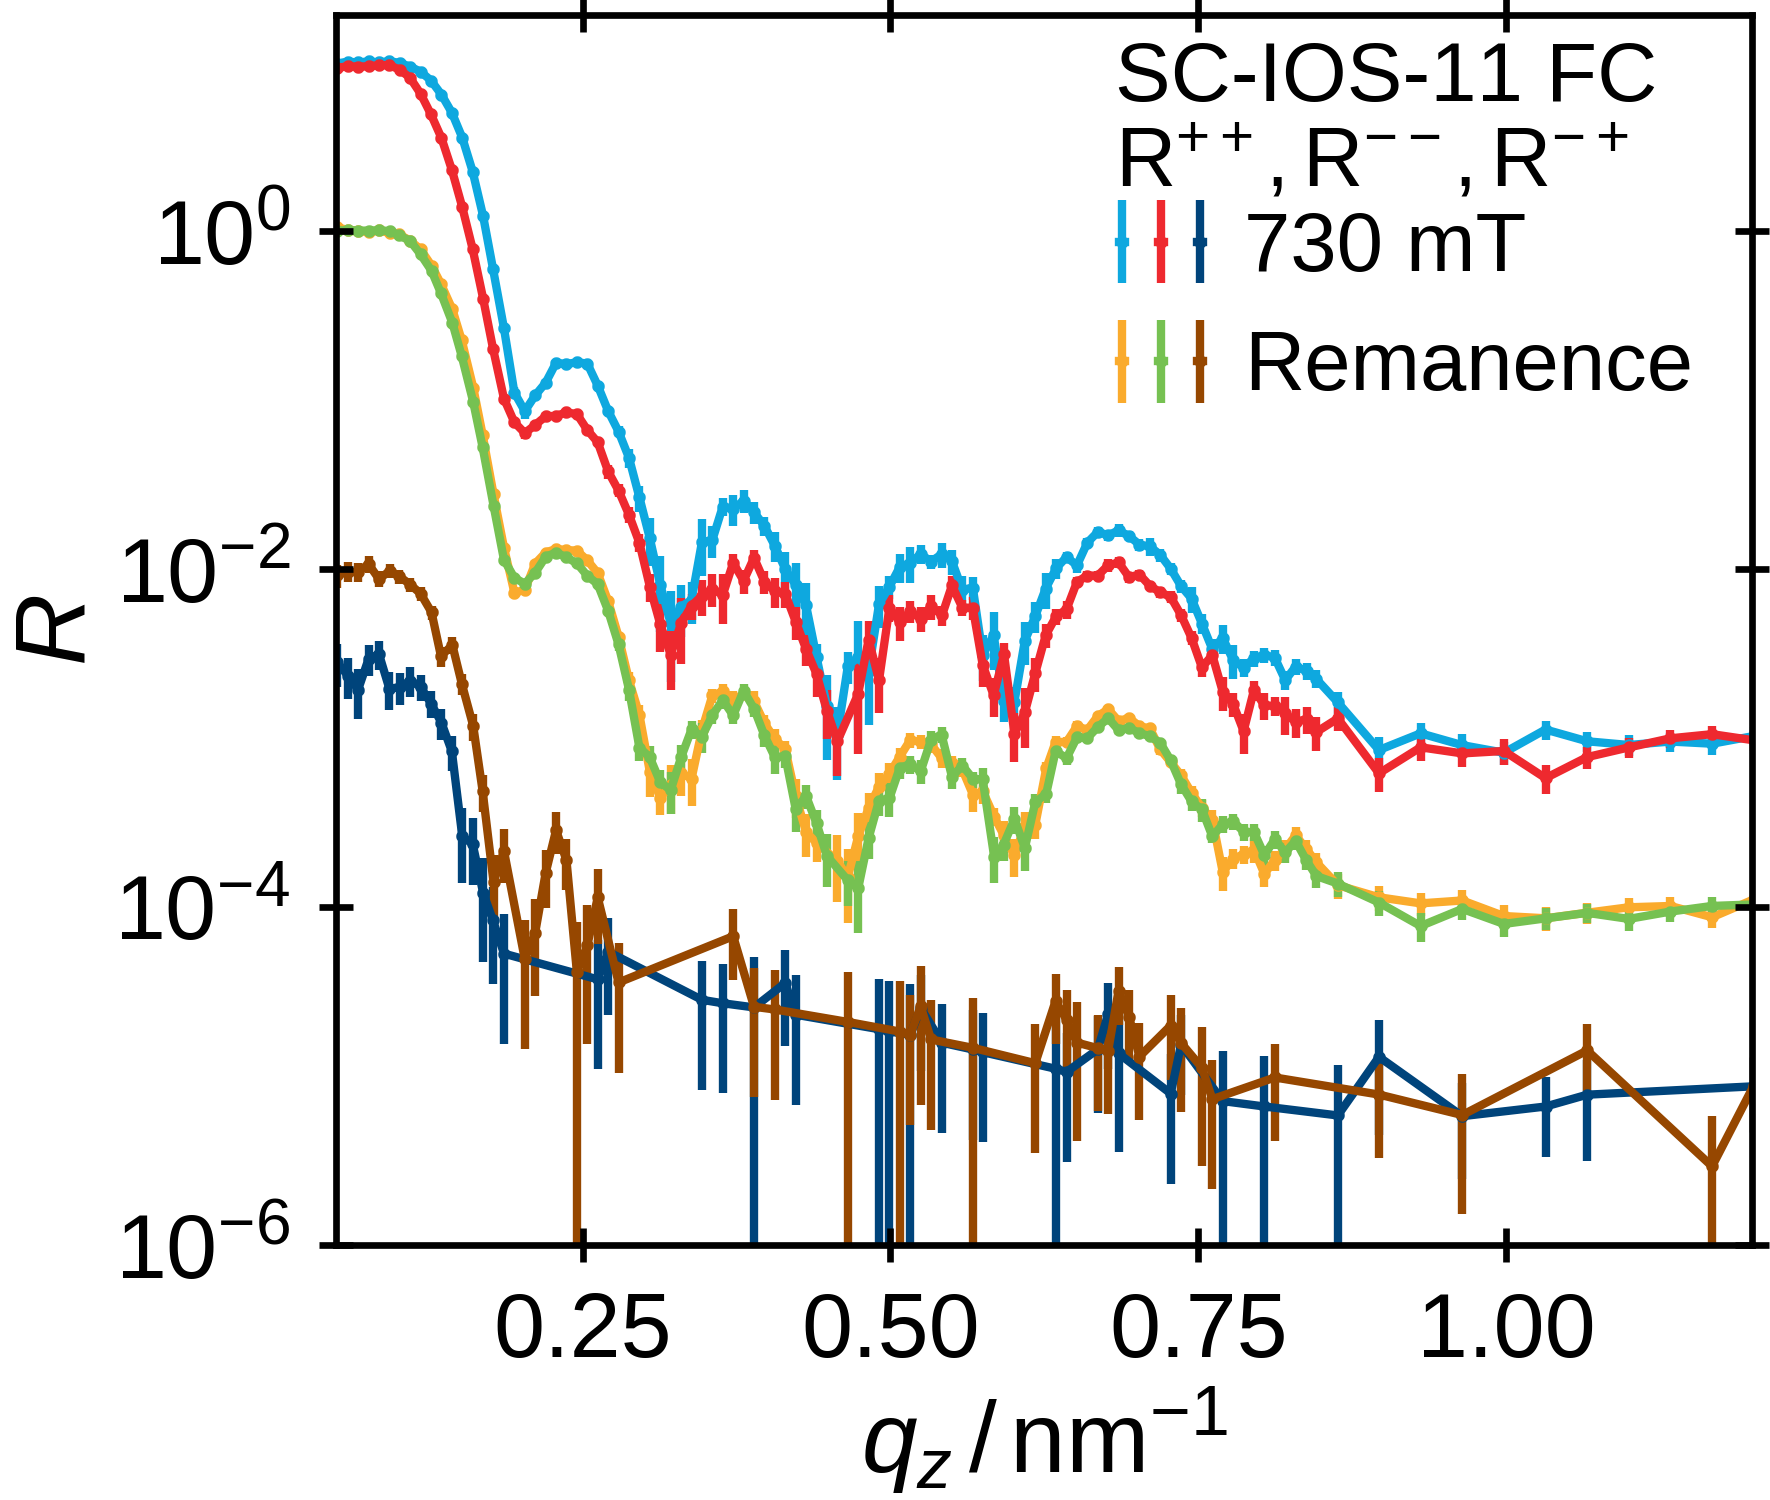
\includegraphics{looselyPackedNP_VerticalStructure_SC-IOS-11_PNR_FC30K}
    \caption{\label{fig:looselyPackedNP:layer:pnrZFCFCIOS11}Zero-field-cooled (left) and Field-cooled non-spin-flip reflectivity ($R^{++},\,R^{--}$) and spin-flip reflectivity ($R^{-+}$) of SC-IOS-11 at a magnetic field of $730 \unit{mT}$ and in remanence. For the zero-field cooled the initial reflectivity after cooling at guide field is additionally shown.}
  \end{figure}

  \begin{figure}[tb]
    \centering
    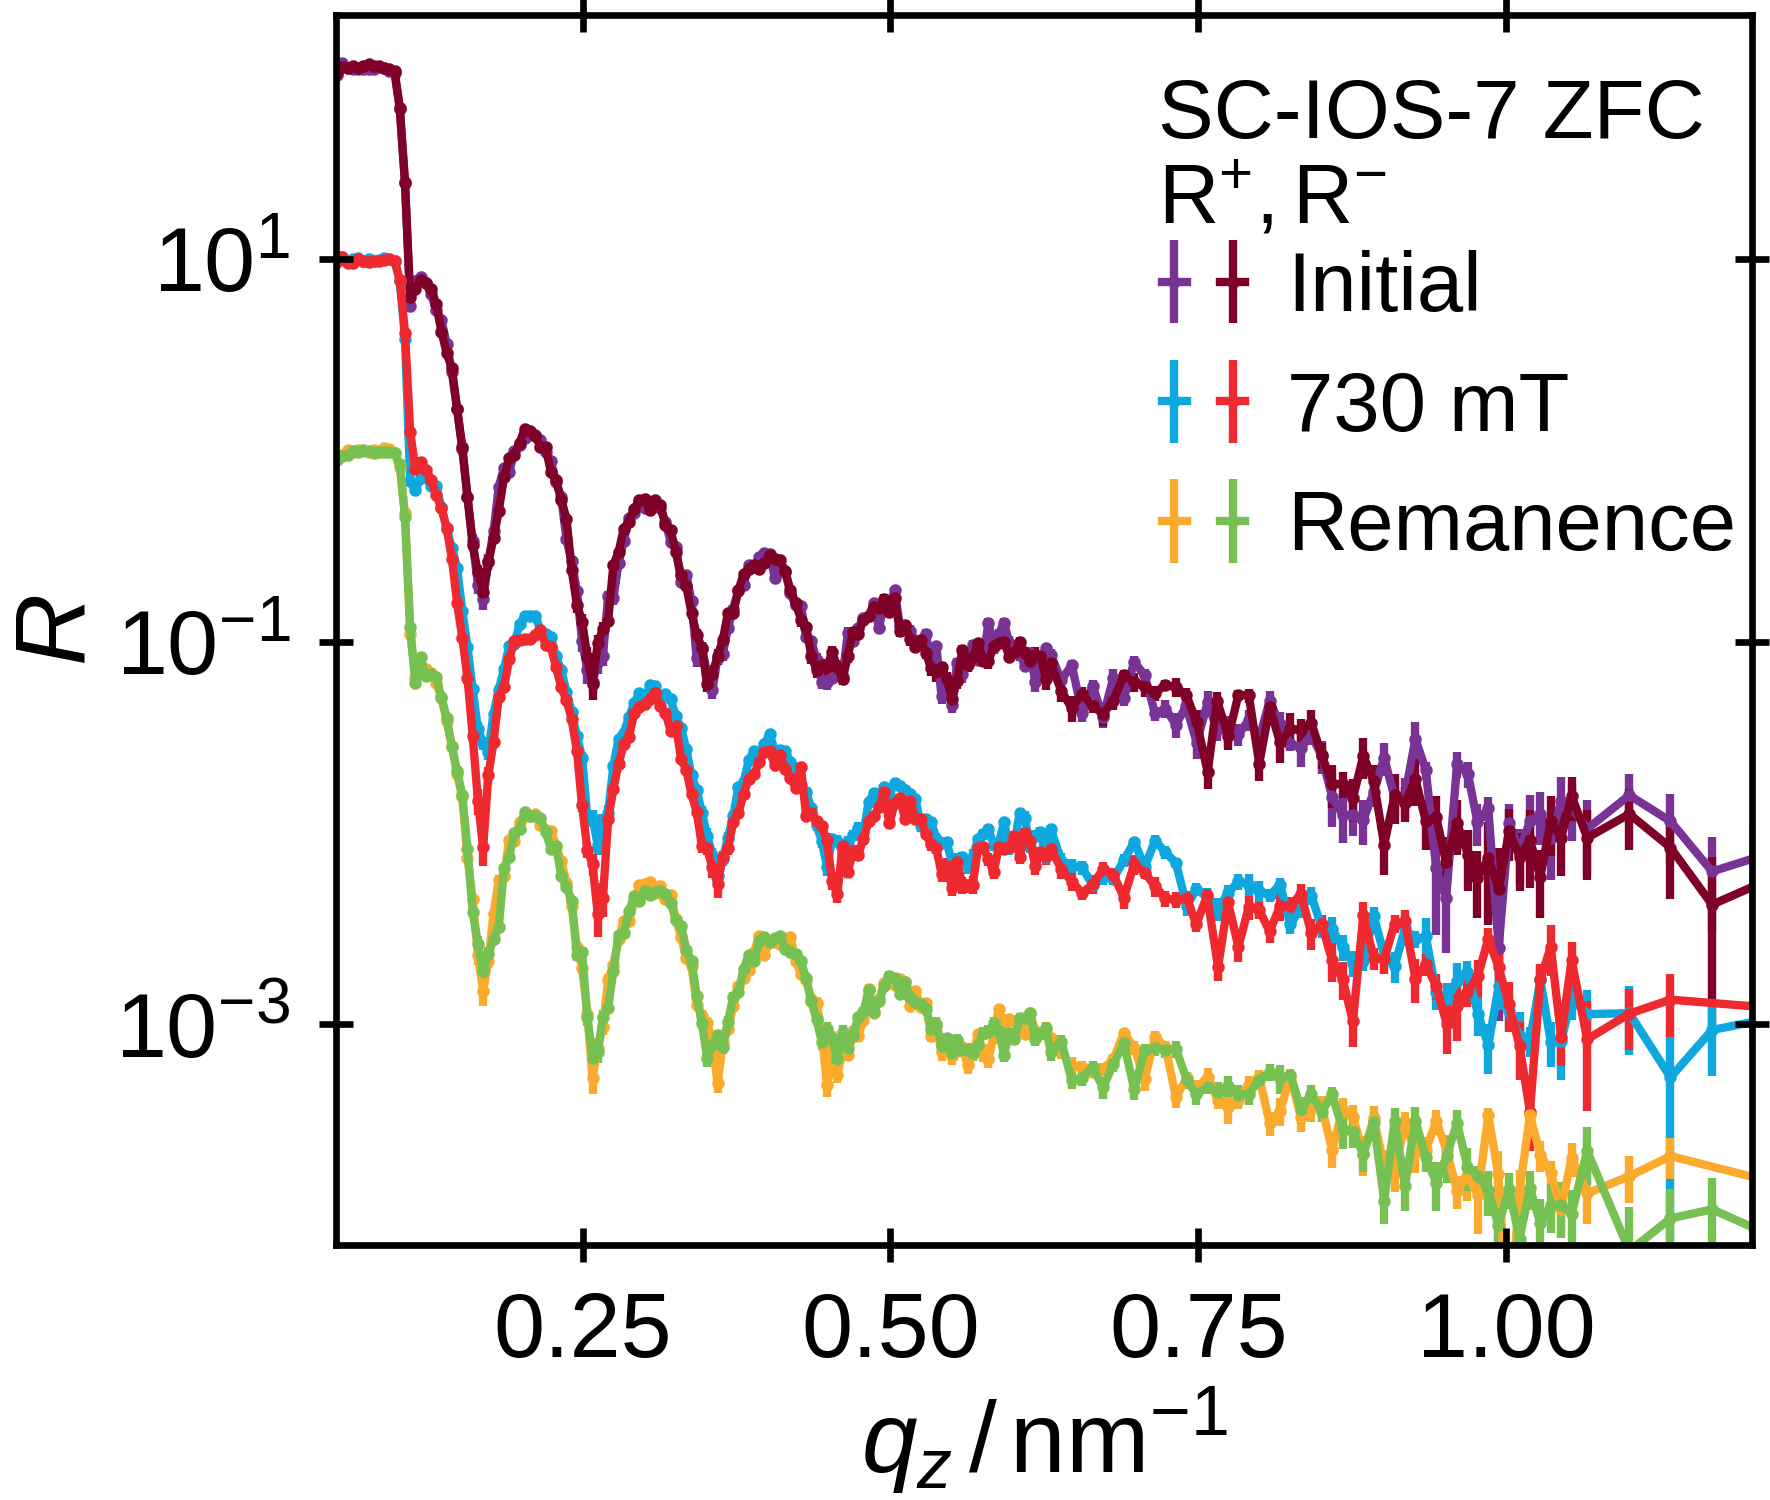
\includegraphics{looselyPackedNP_VerticalStructure_SC-IOS-7_PNR_ZFC30K}
    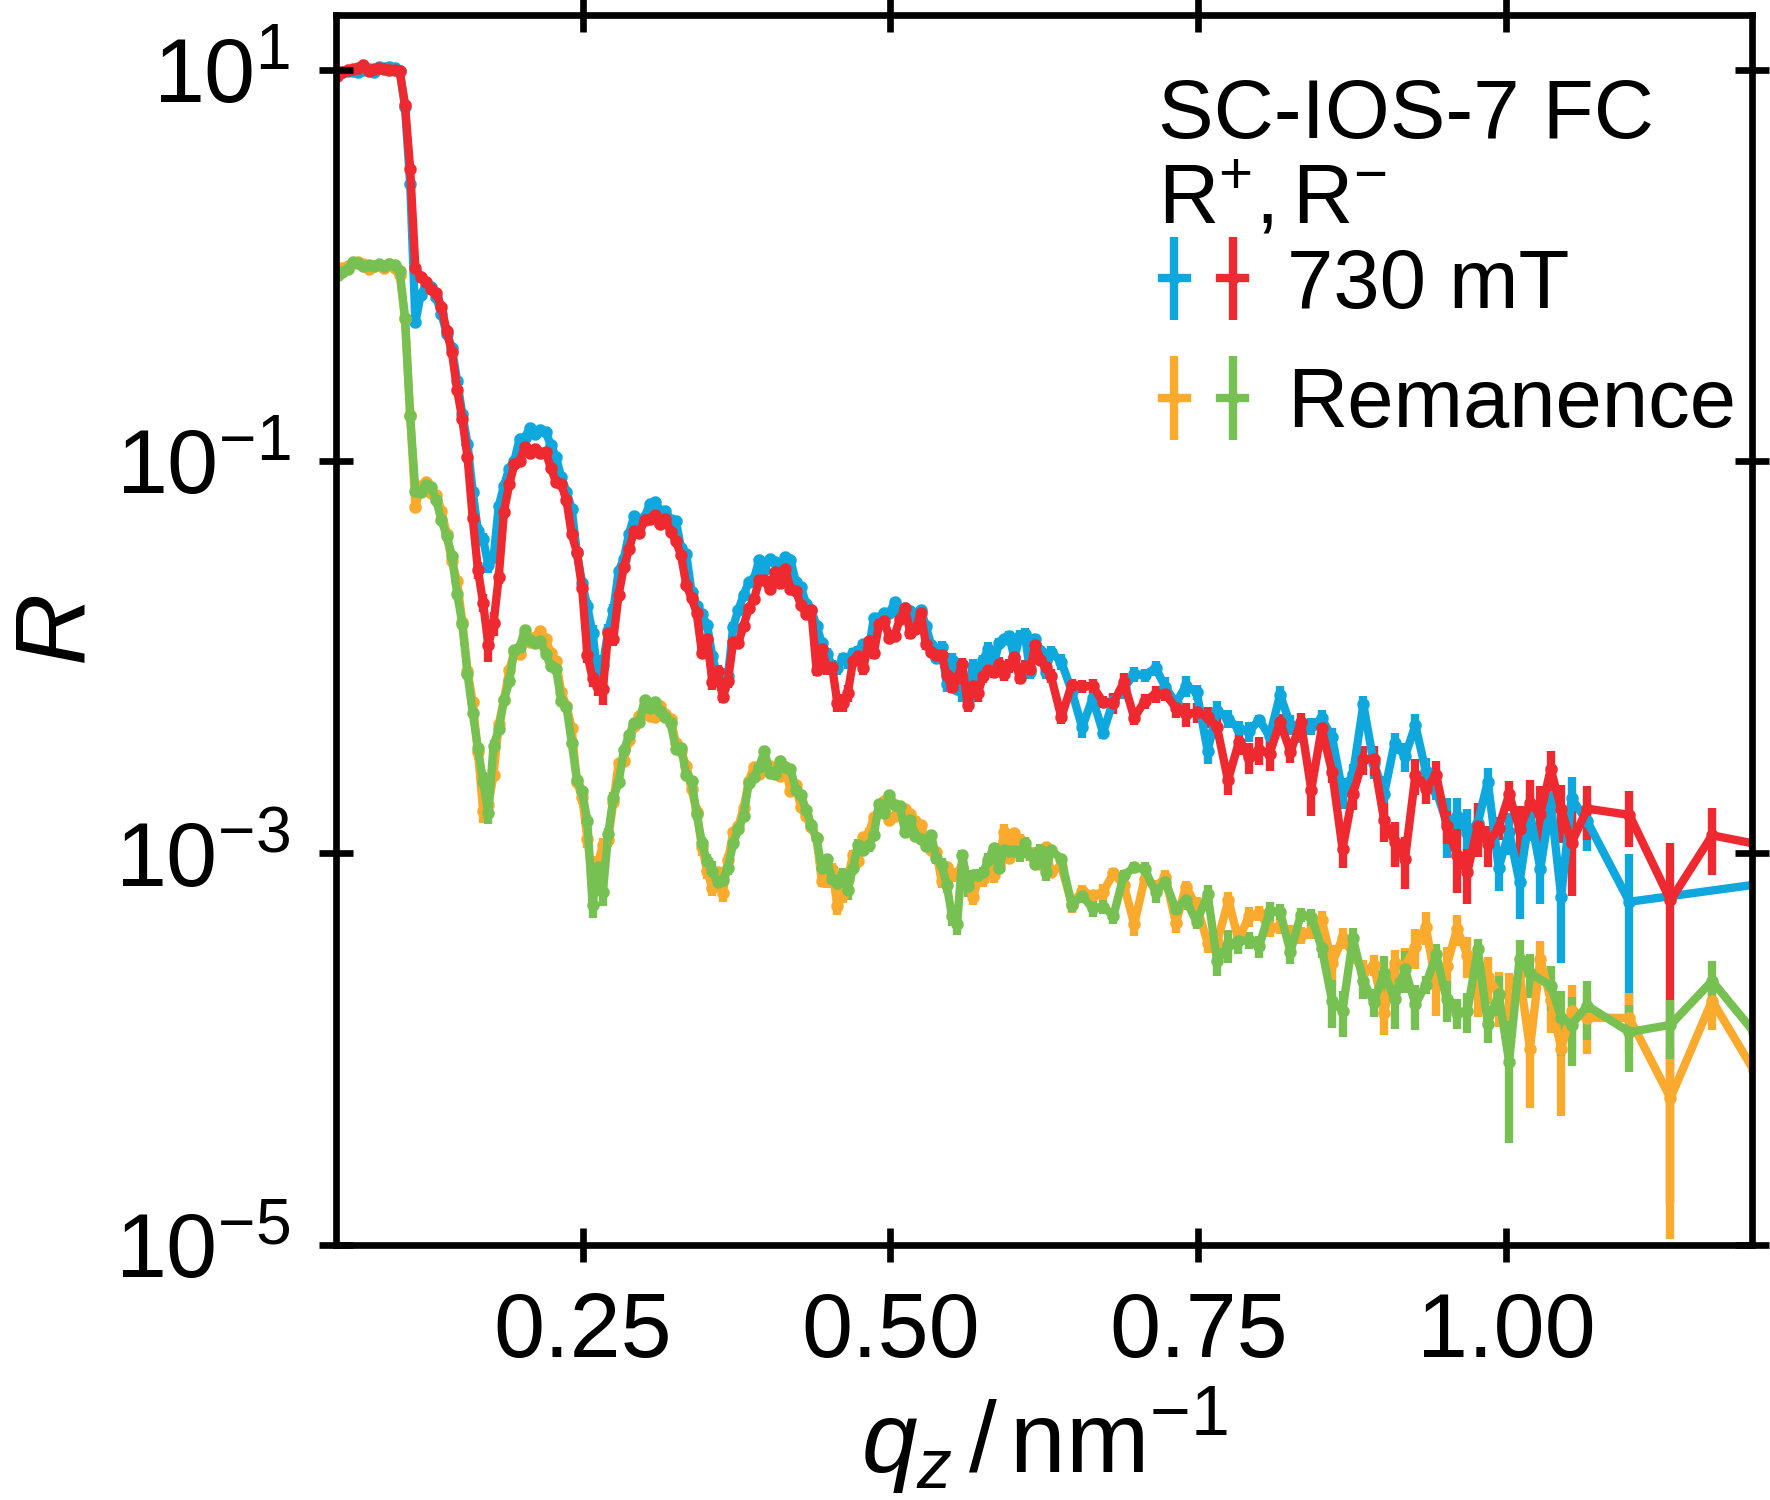
\includegraphics{looselyPackedNP_VerticalStructure_SC-IOS-7_PNR_FC30K}
    \caption{\label{fig:looselyPackedNP:layer:ZFCFCIOS7}Zero-field-cooled (left) and Field-cooled reflectivity of SC-IOS-7 at a magnetic field of $730 \unit{mT}$ and in remanence. For the zero-field cooled the initial reflectivity after cooling at guide field is additionally shown.}
  \end{figure}
\end{document}